\begin{frame}{Polar Plot}
\begin{center}
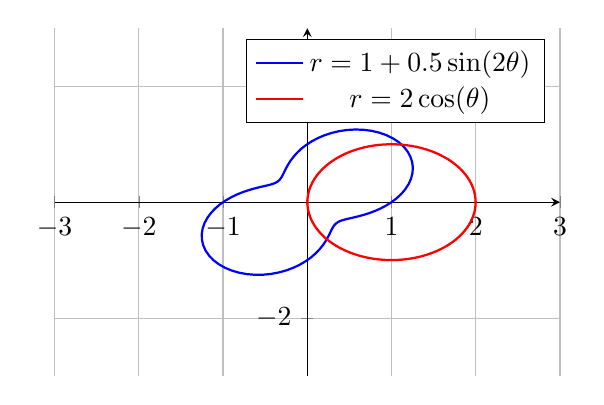
\begin{tikzpicture}
\begin{axis}[
    width=8cm,
    height=6cm,
    grid=both,
    legend pos=north east,
    axis lines=center,
    xmin=-3, xmax=3,
    ymin=-3, ymax=3
]
\addplot[thick, blue, domain=0:360, samples=100] ({cos(x)*(1 + 0.5*sin(2*x))}, {sin(x)*(1 + 0.5*sin(2*x))});
\addplot[thick, red, domain=0:360, samples=100] ({cos(x)*2*cos(x)}, {sin(x)*2*cos(x)});
\legend{$r = 1 + 0.5\sin(2\theta)$, $r = 2\cos(\theta)$}
\end{axis}
\end{tikzpicture}
\end{center}

\footnotesize
Polar plot converted to parametric form
\end{frame}